\documentclass{standalone}
\usepackage{tikz}
\usepackage{ctex,siunitx,ninecolors}
\setCJKmainfont{Noto Serif CJK SC}
\usepackage{tkz-euclide}
\usepackage{amsmath}
\usetikzlibrary{patterns, calc}
\usetikzlibrary {decorations.pathmorphing, decorations.pathreplacing, decorations.shapes,}
\begin{document}
\small
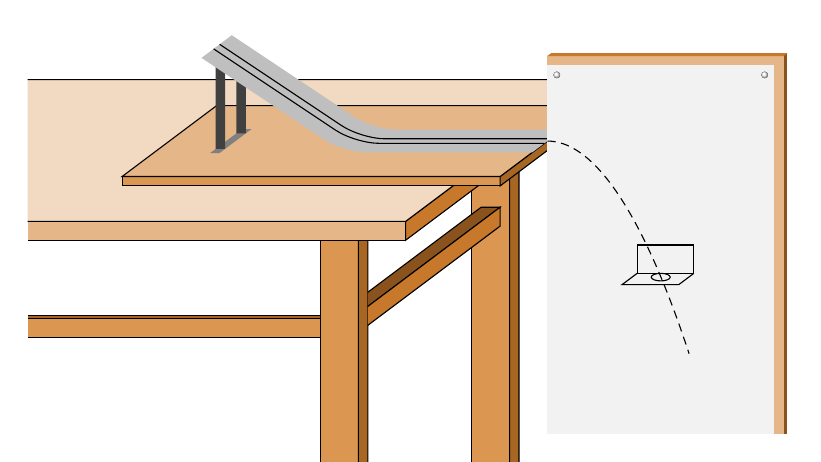
\begin{tikzpicture}[>=stealth,scale=1.2]
  \useasboundingbox(-5,1.5)rectangle(3.1,-2.8);
  \draw[fill=brown5](-5,-1.5475)--(-1.8,-1.5475)--(-1.8,-1.5775)--(-5,-1.5775);
  \draw[fill=brown7](-5,-1.7775)--(-1.8,-1.7775)--(-1.8,-1.5775)--(-5,-1.5775);
  \draw[fill=brown7](-1.9,-0.75)rectangle(-1.5,-4.75)(-0.3,0.6)rectangle(0.1,-3.55);
  \draw[fill=brown5](-1.5,-0.75)--(-1.5,-4.75)--(-1.4,-4.675)--(-1.4,-0.75)(0.1,0.6)--(0.1,-3.55)--(0.2,-3.475)--(0.2,0.675);
  \draw[fill=brown8](-5,-0.75)--(-1,-0.75)--(-1,-0.55)--(-5,-0.55);
  \draw[fill=brown6](-1,-0.75)--(-1,-0.55)--(1,0.95)--(1,0.75)--cycle;
  \draw[fill=brown9](-5,-0.55)--(-1,-0.55)--(1,0.95)--(-5,0.95);
  \draw[fill=brown4](-1.4,-1.3)--(-0.2,-0.4)--(0,-0.4)--(-1.4,-1.45);
  \draw[fill=brown6](-1.4,-1.65)--(0,-0.6)--(0,-0.4)--(-1.4,-1.45);
  \begin{scope}[yshift=2mm,xshift=5mm]
    \draw[fill=brown7](-4.5,-0.375)rectangle(-0.5,-0.275);
    \draw[fill=brown5](-0.5,-0.375)--(-0.5,-0.275)--(0.5,0.475)--(0.5,0.375)--cycle;
    \draw[fill=brown8](-4.5,-0.275)--(-0.5,-0.275)--(0.5,0.475)--(-3.5,0.475)--cycle;
    \fill[gray](-3.57,-0.0275)--(-3.47,-0.0275)--(-3.13,0.2275)--(-3.23,0.2275);
    \fill[darkgray](-3.51,0.0175)rectangle(-3.41,0.9)(-3.29,0.1825)rectangle(-3.19,0.9);
    \fill[lightgray](-0.16,-0.02)[rounded corners=3mm]--(-2.16,-0.02)[sharp corners]--(-3.66,0.98)--(-3.34,1.22)[rounded corners=3mm]--(-1.84,0.22)[sharp corners]--(0.16,0.22);
    \draw[rounded corners=3mm](0.032,0.124)--++(-2,0)--++(-1.5,1.0);
    \draw[rounded corners=3mm](-0.032,0.076)--++(-2,0)--++(-1.5,1.0);
    \fill[brown8](0,1.0)rectangle(2.5,-3);
    \fill[brown4](2.54,1.03)rectangle(2.5,-3);
    \fill[brown6](0,1)--(0.04,1.03)--(2.54,1.03)--(2.5,1);
    \fill[lightgray!20](0,0.9)rectangle(2.4,-3);
    \draw[densely dashed](0,0.1)parabola(1.5,-2.15);
    \draw(1.2,-1.34)ellipse(0.1 and 0.04);
    \draw(0.95,-1.3)rectangle(1.55,-1.0);
    \draw(0.95,-1.3)--++(-0.16,-0.12)--++(0.6,0)--++(0.16,0.12);
    \fill[ball color=white](0.1,0.8)circle(1pt);
    \fill[ball color=white](2.3,0.8)circle(1pt);
  \end{scope}
\end{tikzpicture}
\end{document}